% !TEX root
% Copyright (c) 2021  UAVCAN Consortium <uavcan.org>

\documentclass{uavcandoc}

\usepackage{multirow}
\usepackage{tabularx}
\usepackage{amsmath}
\usepackage{amssymb}
\usepackage{amsfonts}

\urlstyle{same}

\graphicspath{{fig/}}

\title{UAVCAN/CAN Physical Layer Specification v1.0}

\hbadness=10000

\begin{document}
\frontmatter

\begin{titlepage}

\section*{Overview}

The UAVCAN/CAN physical layer specification (UCANPHY) defines electromechanical conventions for {UAVCAN/CAN}
optimized for use in the avionics of manned and unmanned aircraft as well as in high-integrity robotic systems.
The goal of UCANPHY is to maximize cross-vendor compatibility, ensure consistency across the ecosystem, and
prevent some common design pitfalls.

UAVCAN is an open technology for real-time intravehicular distributed computing and communication
based on modern networking standards.
The name UAVCAN stands for \emph{Uncomplicated Application-level Vehicular Computing And Networking}.

UAVCAN/CAN is a standard transport layer protocol defined by the UAVCAN specification for use with
the CAN\footnote{Controller Area Network} protocol.

\BeginRightColumn

\section*{License}

This standard is open to everyone, and it will always remain this way.
No authorization or approval of any kind is necessary for its implementation, distribution, or use.

% The following statement looks a bit archaic, but it is the recommended form according to
% https://creativecommons.org/choose/results-one?license_code=by&amp;jurisdiction=&amp;version=4.0&amp;lang=en
This work is licensed under the Creative Commons Attribution 4.0 International License.
To view a copy of this license, visit
\href{http://creativecommons.org/licenses/by/4.0/}{creativecommons.org/licenses/by/4.0}
or send a letter to Creative Commons, PO Box 1866, Mountain View, CA 94042, USA.

\hspace*{\fill}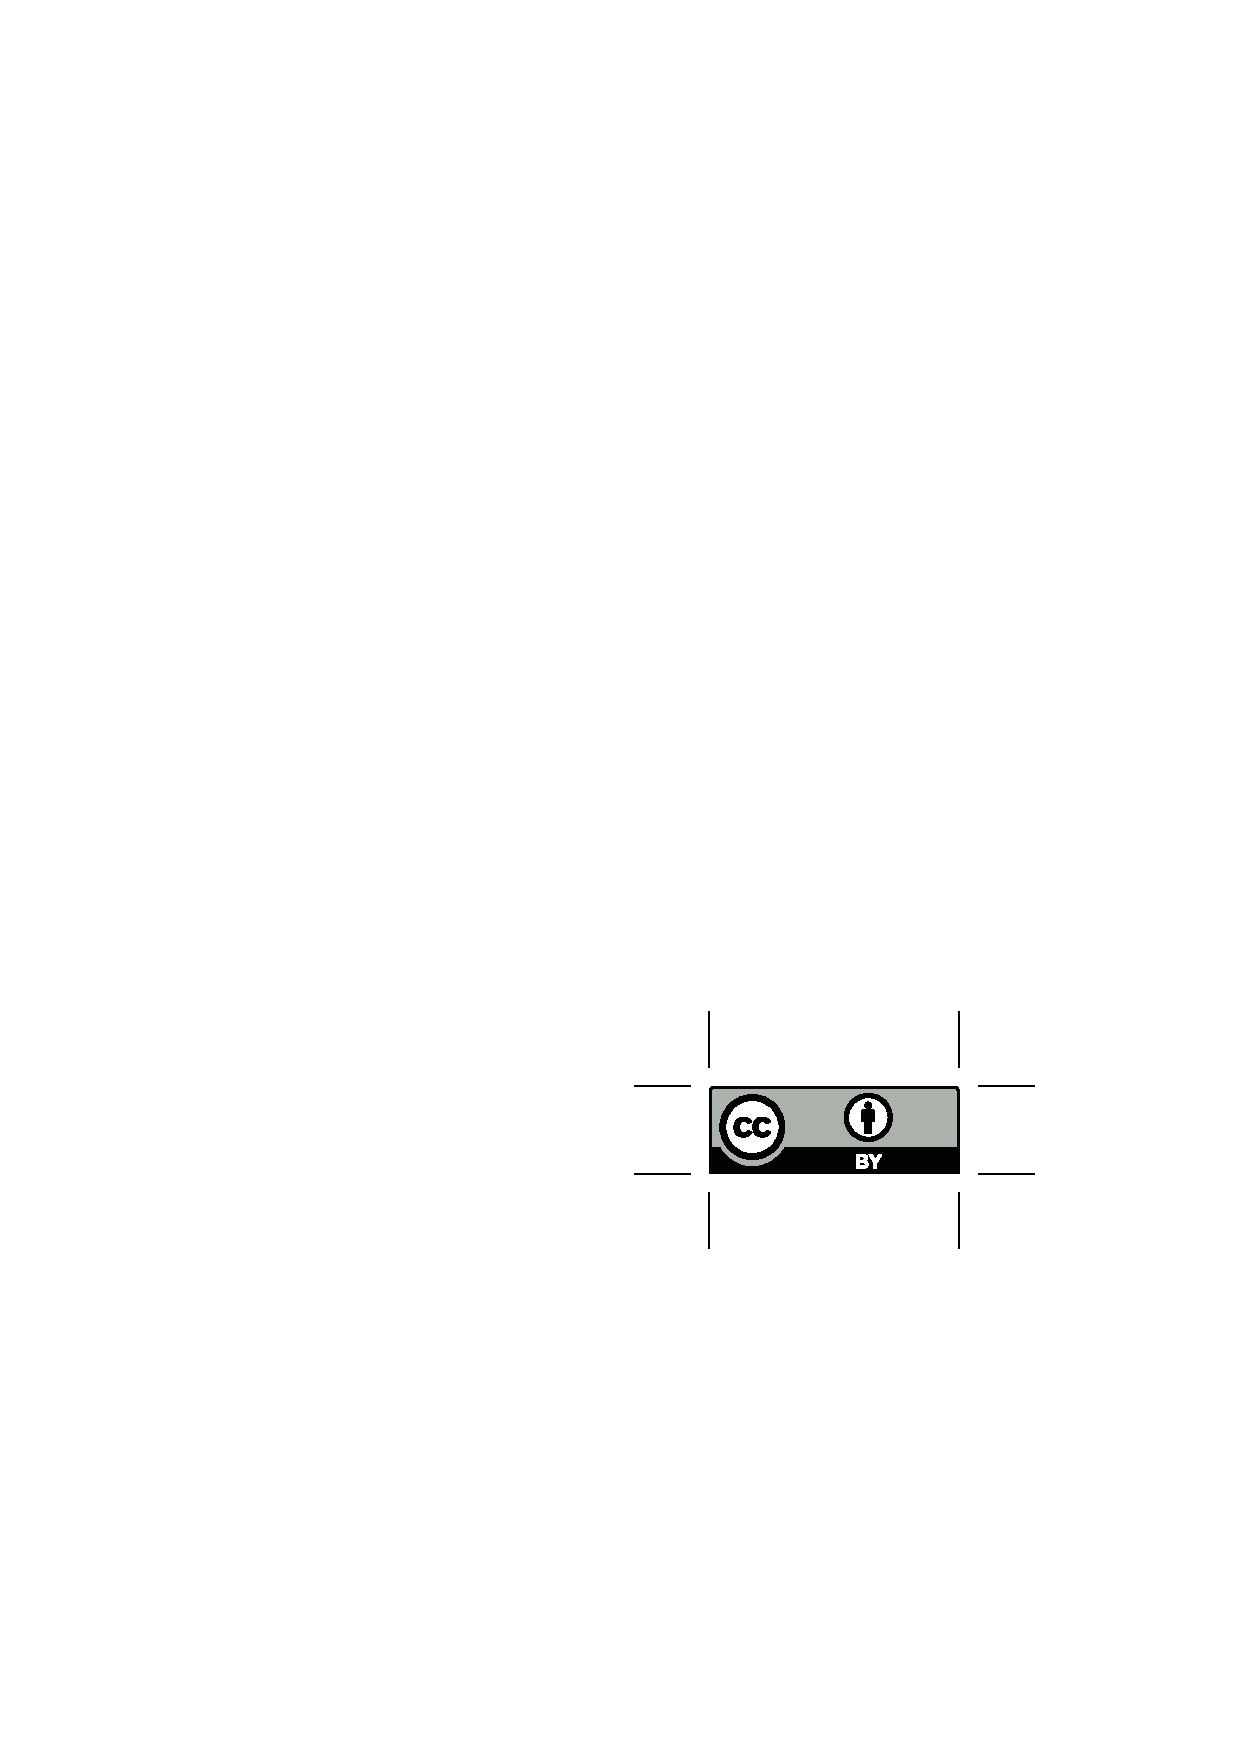
\includegraphics[height=1.75\baselineskip]{cc-by}\hspace*{\fill}

\section*{Disclaimer of warranty}

Note well: this Specification is provided on an ``as is'' basis, without warranties or conditions of any kind,
express or implied, including, without limitation, any warranties or conditions of
title, non-infringement, merchantability, or fitness for a particular purpose.

\section*{Limitation of liability}

In no event and under no legal theory, whether in tort (including negligence), contract, or otherwise,
unless required by applicable law (such as deliberate and grossly negligent acts) or agreed to in writing,
shall any author of this Specification be liable for damages,
including any direct, indirect, special, incidental, or consequential damages of any character arising
from, out of, or in connection with the Specification or the implementation, deployment,
or other use of the Specification (including but not limited to damages for loss of goodwill,
work stoppage, equipment failure or malfunction, injuries to persons, death,
or any and all other commercial damages or losses),
even if such author has been made aware of the possibility of such damages.

\end{titlepage}

\tableofcontents
\BeginRightColumn
\listoftables
\listoffigures

\mainmatter

\chapter{Introduction}\label{sec:introduction}

This is a non-normative chapter covering the basic concepts that govern development and maintenance of
the specification.

\section{Overview}

The UAVCAN/CAN physical layer specification (UCANPHY) defines electromechanical conventions for {UAVCAN/CAN}
optimized for use in the avionics of manned and unmanned aircraft as well as in high-integrity robotic systems.
The goal of UCANPHY is to maximize cross-vendor compatibility, ensure consistency across the ecosystem, and
prevent some common design pitfalls.

The development and maintenance of the UCANPHY specification is carried out by the members of the UAVCAN Consortium.
Information on the Consortium is available via the official website at \href{http://uavcan.org}{uavcan.org}.

Information on UAVCAN and its CAN-based transport named UAVCAN/CAN is published in a separate document
available from the official website.

\section{Document conventions}

Non-normative text, examples, recommendations, elaborations, and other optional items
are contained in footnotes\footnote{This is a footnote.} or highlighted sections as shown below.

\begin{remark}
    Non-normative sections such as examples are enclosed in shaded boxes like this.
\end{remark}

Throughout the document, ``CAN'' implies both Classic CAN and CAN FD, unless specifically noted otherwise.

\section{Management and conformance}

The UAVCAN Consortium is tasked with maintaining and advancing this specification,
as well as performing voluntary conformance testing.
The policies that govern these activities are published on the official website.

Products whose conformance with this specification has been confirmed by the Consortium
are entitled to feature the official \emph{UAVCAN Conformity Mark}
subject to the policies published on the official website.

\section{Referenced sources}

The specification contains references to the following sources:

% Please keep the list sorted alphabetically.
\begin{itemize}
    \item CiA 103 --- Intrinsically safe capable physical layer.
    \item CiA 801 --- Application note --- Automatic bit rate detection.

    \item IETF RFC2119 --- Key words for use in RFCs to Indicate Requirement Levels.

    \item ISO 11898-1 --- Controller area network (CAN) --- Part 1: Data link layer and physical signaling.
    \item ISO 11898-2 --- Controller area network (CAN) --- Part 2: High-speed medium access unit.
\end{itemize}

\section{Revision history}

\subsection{v1.0 -- Oct 2021}

This is the first revision of the standard.

\chapter{CAN bus physical layer}\label{sec:phy}

As can be seen from its specification, UAVCAN is mostly agnostic of the parameters of the physical layer.
Despite that, vendors should follow the recommendations provided in this section
in the interest of maximizing the cross-vendor compatibility.

\section{Classic CAN}

Table~\ref{table:phy_parameters_classic_can} lists the recommended parameters of the
ISO 11898-2 Classic CAN physical layer.
The estimated bus length limits are based on the assumption that the propagation delay does not exceed 5 ns/m,
not including additional delay times of CAN transceivers and other components.

\begin{UAVCANSimpleTable}[wide]{ISO 11898-2 Classic CAN physical layer parameters}{|l| X[c] X[c] X[c] X[c] |l|}%
    \label{table:phy_parameters_classic_can}%
    Parameter                           &           \multicolumn{4}{c|}{Value}          & Unit      \\
    Bit rate                            &   1000    &   500     &   250     &   125     & kbit/s    \\
    Permitted sample point location     &   75--90  &   85--90  &   85--90  &   85--90  & \%        \\
    Recommended sample point location   &   87.5    &   87.5    &   87.5    &   87.5    & \%        \\
    Maximum bus length                  &   40      &   100     &   250     &   500     & m         \\
    Maximum stub length                 &   0.3     &   0.3     &   0.3     &   0.3     & m         \\
\end{UAVCANSimpleTable}

Designers are encouraged to implement CAN auto bit rate detection when applicable.
Refer to the CiA 801 application note for the recommended practices.

\begin{remark}
    UAVCAN allows the use of a simple bit time measuring approach,
    as it is guaranteed that any functioning UAVCAN network will always exchange node status messages,
    which can be expected to be published at a rate no lower than 1 Hz,
    and that contain a suitable alternating bit pattern in the CAN ID field.
    Refer to the UAVCAN Specification for details.
\end{remark}

\section{CAN FD}

This section is under development and will be populated in a later revision of the document.

\begin{table}[H]
    \caption{ISO 11898-2 CAN FD physical layer parameters}
    \NoLeftSkip
    \begin{tabu} to \textwidth {|l l| X[c] X[c] X[c] X[c] |l|}
        \hline\rowfont{\bfseries{}}
        \label{table:phy_parameters_can_fd}%
        Parameter                           & Segment       & \multicolumn{4}{c|}{Value}& Unit \\\hline

        \multirow{2}{*}{Bit rate}           & Arbitration   & 1000 & 500  & 250  & 125  & \multirow{2}{*}{kbit/s} \\
                                            & Data          & 4000 & 2000 & 1000 & 500  &                       \\\hline
        \multirow{2}{*}{Permitted SPL}      & Arbitration   & TBD  & TBD  & TBD  & TBD  & \multirow{2}{*}{\%}   \\
                                            & Data          & TBD  & TBD  & TBD  & TBD  &                       \\\hline
        \multirow{2}{*}{Recommended SPL}    & Arbitration   & TBD  & TBD  & TBD  & TBD  & \multirow{2}{*}{\%}   \\
                                            & Data          & TBD  & TBD  & TBD  & TBD  &                       \\\hline
        \multicolumn{2}{|l|}{Maximum bus length}            & TBD  & TBD  & TBD  & TBD  & \multirow{2}{*}{m}    \\
        \multicolumn{2}{|l|}{Maximum stub length}           & TBD  & TBD  & TBD  & TBD  &                       \\\hline

    \end{tabu}
\end{table}

\chapter{Connectors}\label{sec:connector}

The UCANPHY standard defines several connector types optimized for different applications:
from highly compact systems to large deployments, from low-cost to safety-critical applications.
Each connector type specification includes an integrated power supply interface
(section~\ref{sec:power}).

Implementations should provide two identical parallel connectors for each CAN interface per device
instead of relying on T-connectors.
T-connectors should be avoided because typically they increase the stub length, weight, and
complexity of the wiring harnesses.
All signals of the paired connectors, including those that are unused, shall be interconnected one to one.

\begin{UAVCANSimpleTable}[wide]{Standard UAVCAN/CAN connector types}{|l l l X|}\label{table:connector_summary}
    Connector name & Base connector type & Integrated power & Known compatible standards \\
    \textbf{UCANPHY D-Sub} &
    Generic D-Subminiature DE-9 &
    24 V, 3 A &
    De-facto standard connector for CAN, supported by many current specifications. \\

    \textbf{UCANPHY M8} &
    Generic M8 5-circuit B-coded &
    24 V, 3 A &
    CiA 103 (CANopen) \\

    \textbf{UCANPHY Micro} &
    JST GH 4-circuit &
    5 V, 1 A &
    Dronecode Autopilot Connector Standard \\
\end{UAVCANSimpleTable}

\clearpage  % Enforce \clearpage because the text here is very graphics-heavy and may be hard to read otherwise
\section{UCANPHY D-Sub}

The UCANPHY D-Sub connector type is based upon, and compatible with, the D-Subminiature DE-9 CAN connector
(this is the most popular CAN connector type, in effect the de-facto industry standard).
This connector is fully compatible with CANopen and many other current specifications.

{
\NoLeftSkip
\begin{UAVCANCompactTable}{|X[2] X|}
    Advantages & Disadvantages \\
    \begin{itemize}
        \item Highest level of compatibility with the existing commercial off the shelf (COTS) hardware.
        Connectors, cables, termination plugs, and other components can be procured from many different vendors.
        \item High-reliability options suitable for safety-critical systems are available from multiple vendors.
        \item Low-cost options are available from multiple vendors.
        \item Both PCB-mounted and panel-mounted types are available.
    \end{itemize}
    &
    D-Subminiature is the largest connector type defined by UCANPHY.
    Due to its significant size and weight, it may be unsuitable for some applications.
\end{UAVCANCompactTable}
}

The UCANPHY D-Sub connector is based on the industry-standard \textbf{D-Sub DE-9} (9-circuit) connector type.
Devices are equipped with the male plug connector type mounted on the panel or on the PCB,
and the cables are equipped with the female socket connectors on both ends
(figure~\ref{fig:connector_d_sub}).

If the device uses two parallel connectors per CAN bus interface (as recommended),
then all of the lines of the paired connectors,
including those that are not used by the current specification,
shall be interconnected one to one.
This will ensure compatibility with future revisions of the specification that make use of
currently unused circuits of the connector.

The CAN physical layer standard that should be used with this connector type is
ISO 11898-2\footnote{Also known as \emph{high-speed CAN}.}.

Devices that deliver power to the bus are required to provide 23.0--30.0 V on the bus power line, 24 V nominal.
Devices that are powered from the bus should expect 18.0--30.0 V on the bus power line.
The current shall not exceed 3 A per connector.

Table~\ref{table:connector_d_sub_pinout} documents the pinout specification for the
UCANPHY D-Sub connector type.
Signals ``CAN High'' and ``CAN Low'' shall belong to the same twisted pair.
Usage of twisted or flat wires for all other signals remains at the discretion of the implementer.

\begin{UAVCANSimpleTable}{UCANPHY D-Sub connector pinout}{|l l X|}\label{table:connector_d_sub_pinout}
    \# & Function           & Note \\
    1  &                    &  \\
    2  & CAN low            & Twisted with ``CAN high'' (pin 7). \\
    3  & CAN ground         & Shall be interconnected with ``Ground'' (pin 6) within the device. \\
    4  &                    &  \\
    5  & CAN shield         & Optional. \\
    6  & Ground             & Shall be interconnected with ``CAN ground'' (pin 3) within the device. \\
    7  & CAN high           & Twisted with ``CAN low'' (pin 2). \\
    8  &                    &  \\
    9  & Bus power supply   & 24 V nominal. See the power supply requirements. \\
\end{UAVCANSimpleTable}

\begin{figure}[hbt]
    \centering
    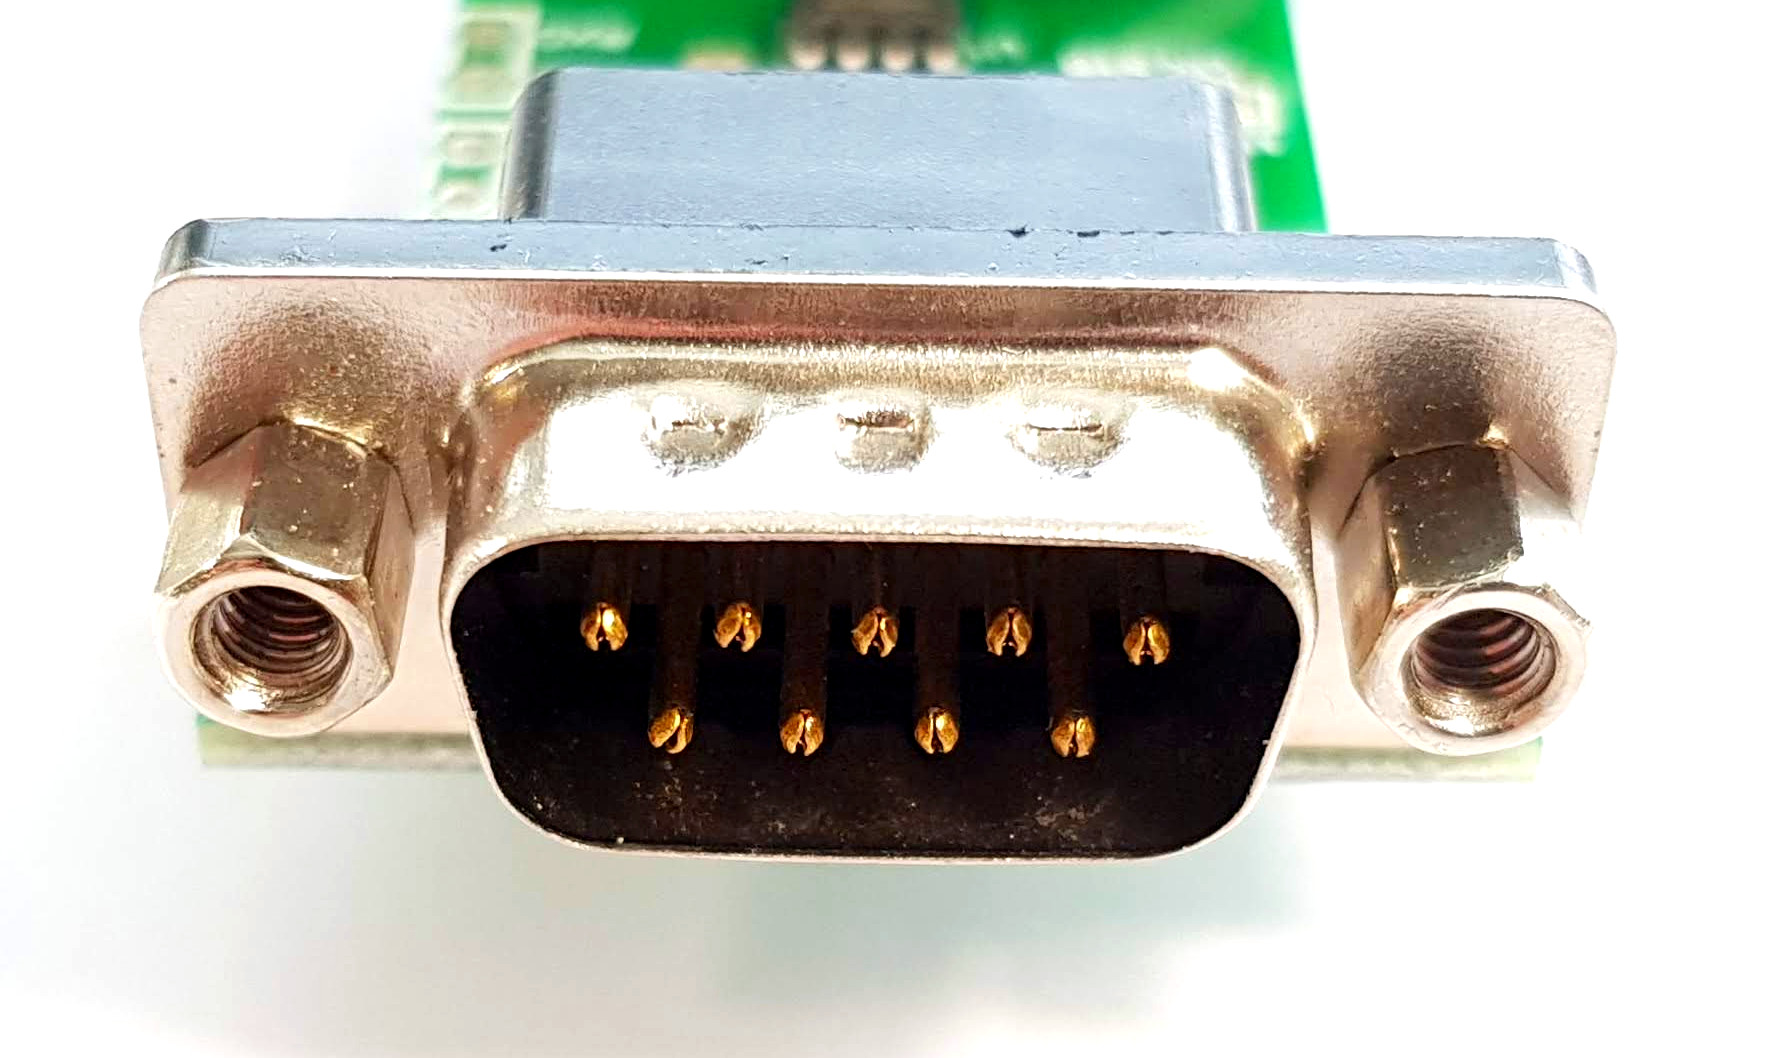
\includegraphics[width=0.35\textwidth]{de-9_connector_male_plug}
    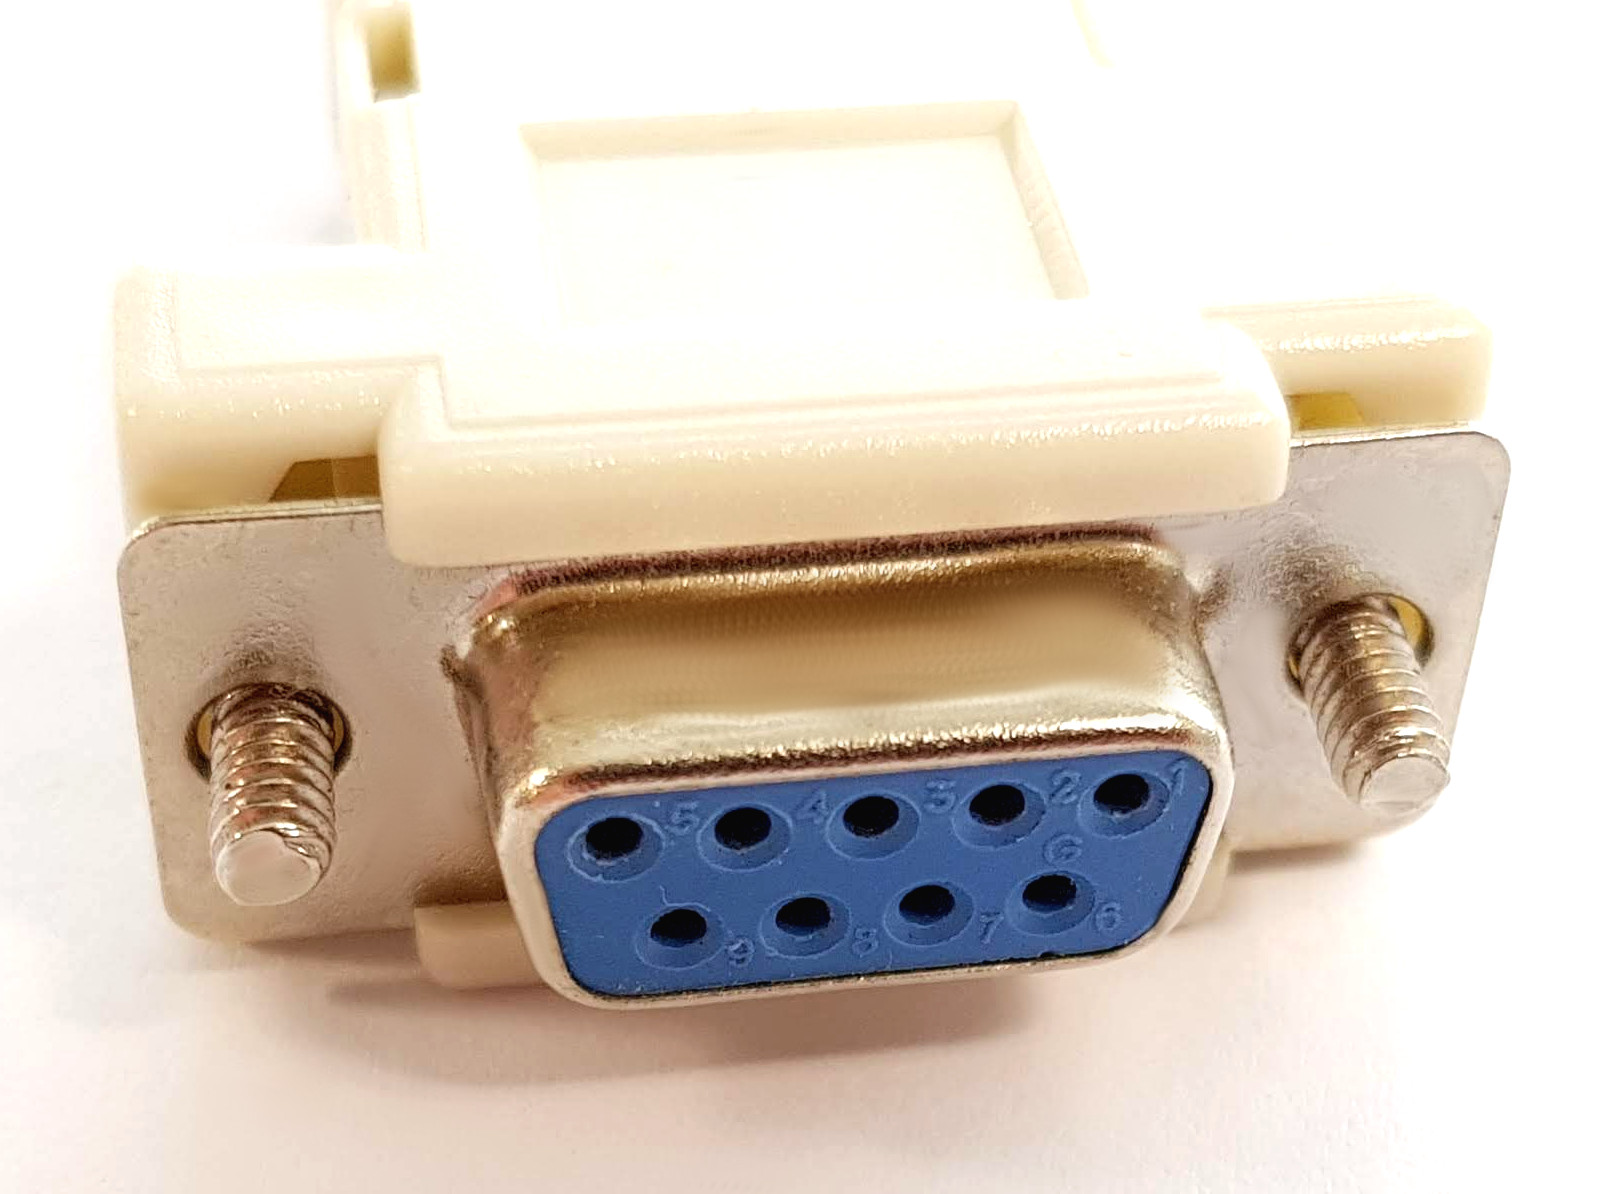
\includegraphics[width=0.35\textwidth]{de-9_cable_female_socket}\\
    Device (left) and cable (right) connectors.
    \caption{UCANPHY D-Sub connectors\label{fig:connector_d_sub}}
\end{figure}

\clearpage  % Enforce \clearpage because the text here is very graphics-heavy and may be hard to read otherwise
\section{UCANPHY M8}

The UCANPHY M8 connector type is based on the generic circular M8 connector type.
This is a popular industry-standard connector; there are multiple vendors that manufacture compatible components:
connectors, cables, termination plugs, T-connectors, and so on.
The pinning, physical layer, and supply voltages used in this connector type are compatible with CiA 103 (CANopen)
and some other CAN bus standards.

{
\NoLeftSkip
\begin{UAVCANCompactTable}{|X[3] X[2]|}
    Advantages & Disadvantages \\
    \begin{itemize}
        \item Compatibility with existing COTS hardware.
        Connectors, cables, termination plugs, and other components can be purchased from many different vendors.
        \item High-reliability options suitable for safety-critical systems are available from multiple vendors.
        \item Low-cost options are available from multiple vendors.
        \item Reasonably compact. M8 connectors are much smaller than D-Sub.
        \item PCB-mounted and panel-mounted types are available.
    \end{itemize}
    &
    \begin{itemize}
        \item M8 connectors may be a poor fit for applications that have severe weight and space constraints.
        \item The level of adoption in the industry is noticeably lower than that of the D-Sub connector type.
    \end{itemize}
\end{UAVCANCompactTable}
}

The UCANPHY M8 connector is based on the \textbf{circular M8 B-coded 5-circuit} connector type\footnote{%
    Do not confuse A-coded and B-coded M8 connectors -- they are not mutually compatible.
}.
Devices are equipped with the male plug mounted on the panel or on the PCB,
and cables are equipped with the female socket on both ends (figure~\ref{fig:connector_m8}).

The CAN physical layer standard that should be used with this connector type is
ISO 11898-2\footnote{Also known as \emph{high-speed CAN}.}.

Devices that deliver power to the bus are required to provide 23.0--30.0 V on the bus power line, 24 V nominal.
Devices that are powered from the bus should expect 18.0--30.0 V on the bus power line.
The current shall not exceed 3 A per connector.

Table~\ref{table:connector_m8_pinout} documents the pinout specification for the UCANPHY M8 connector type.
Wires ``CAN high'' and ``CAN low'' should be a twisted pair.

\begin{UAVCANSimpleTable}{UCANPHY M8 connector pinout}{|l l X|}\label{table:connector_m8_pinout}
    \# & Function           & Note \\
    1  & Bus power supply   & 24 V nominal. See the power supply requirements. \\
    2  & CAN shield         & Optional. \\
    3  & CAN high           & Twisted with ``CAN low'' (pin 4). \\
    4  & CAN low            & Twisted with ``CAN high'' (pin 3). \\
    5  & Ground             & \\
\end{UAVCANSimpleTable}

\begin{figure}[hbt]
    \centering
    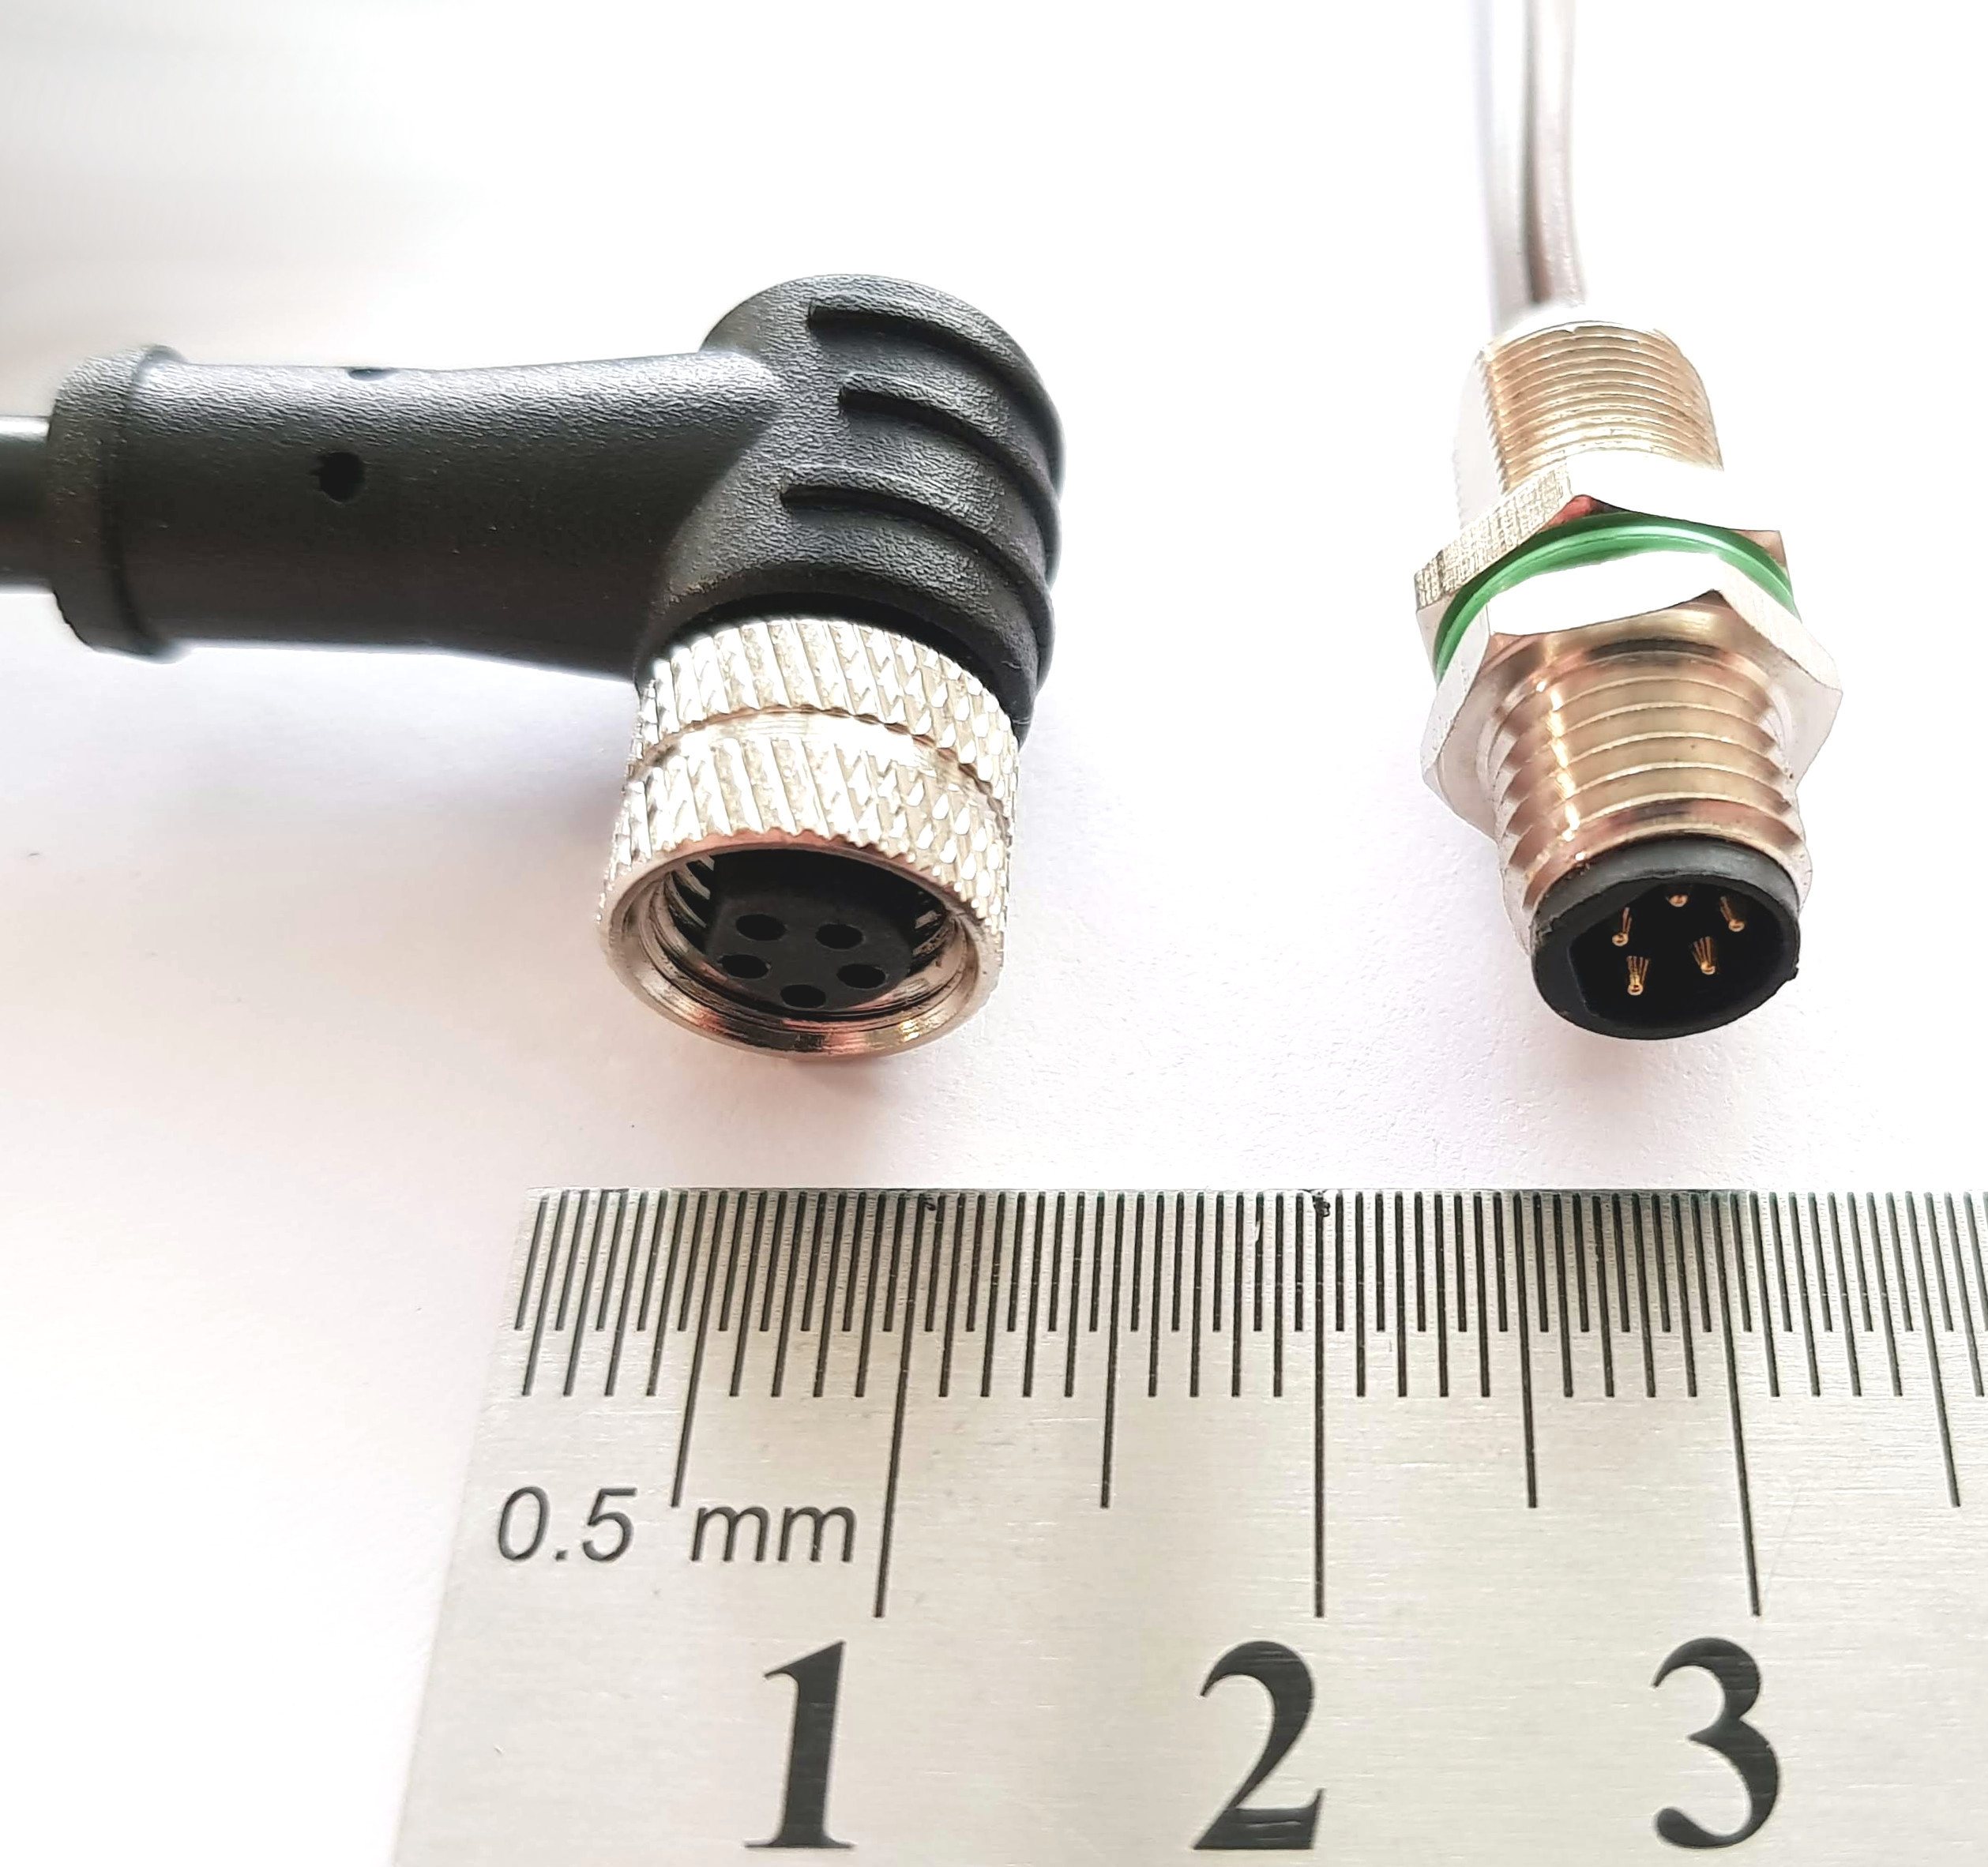
\includegraphics[width=0.35\textwidth]{m8_connector_pair_female_socket_male_plug}
    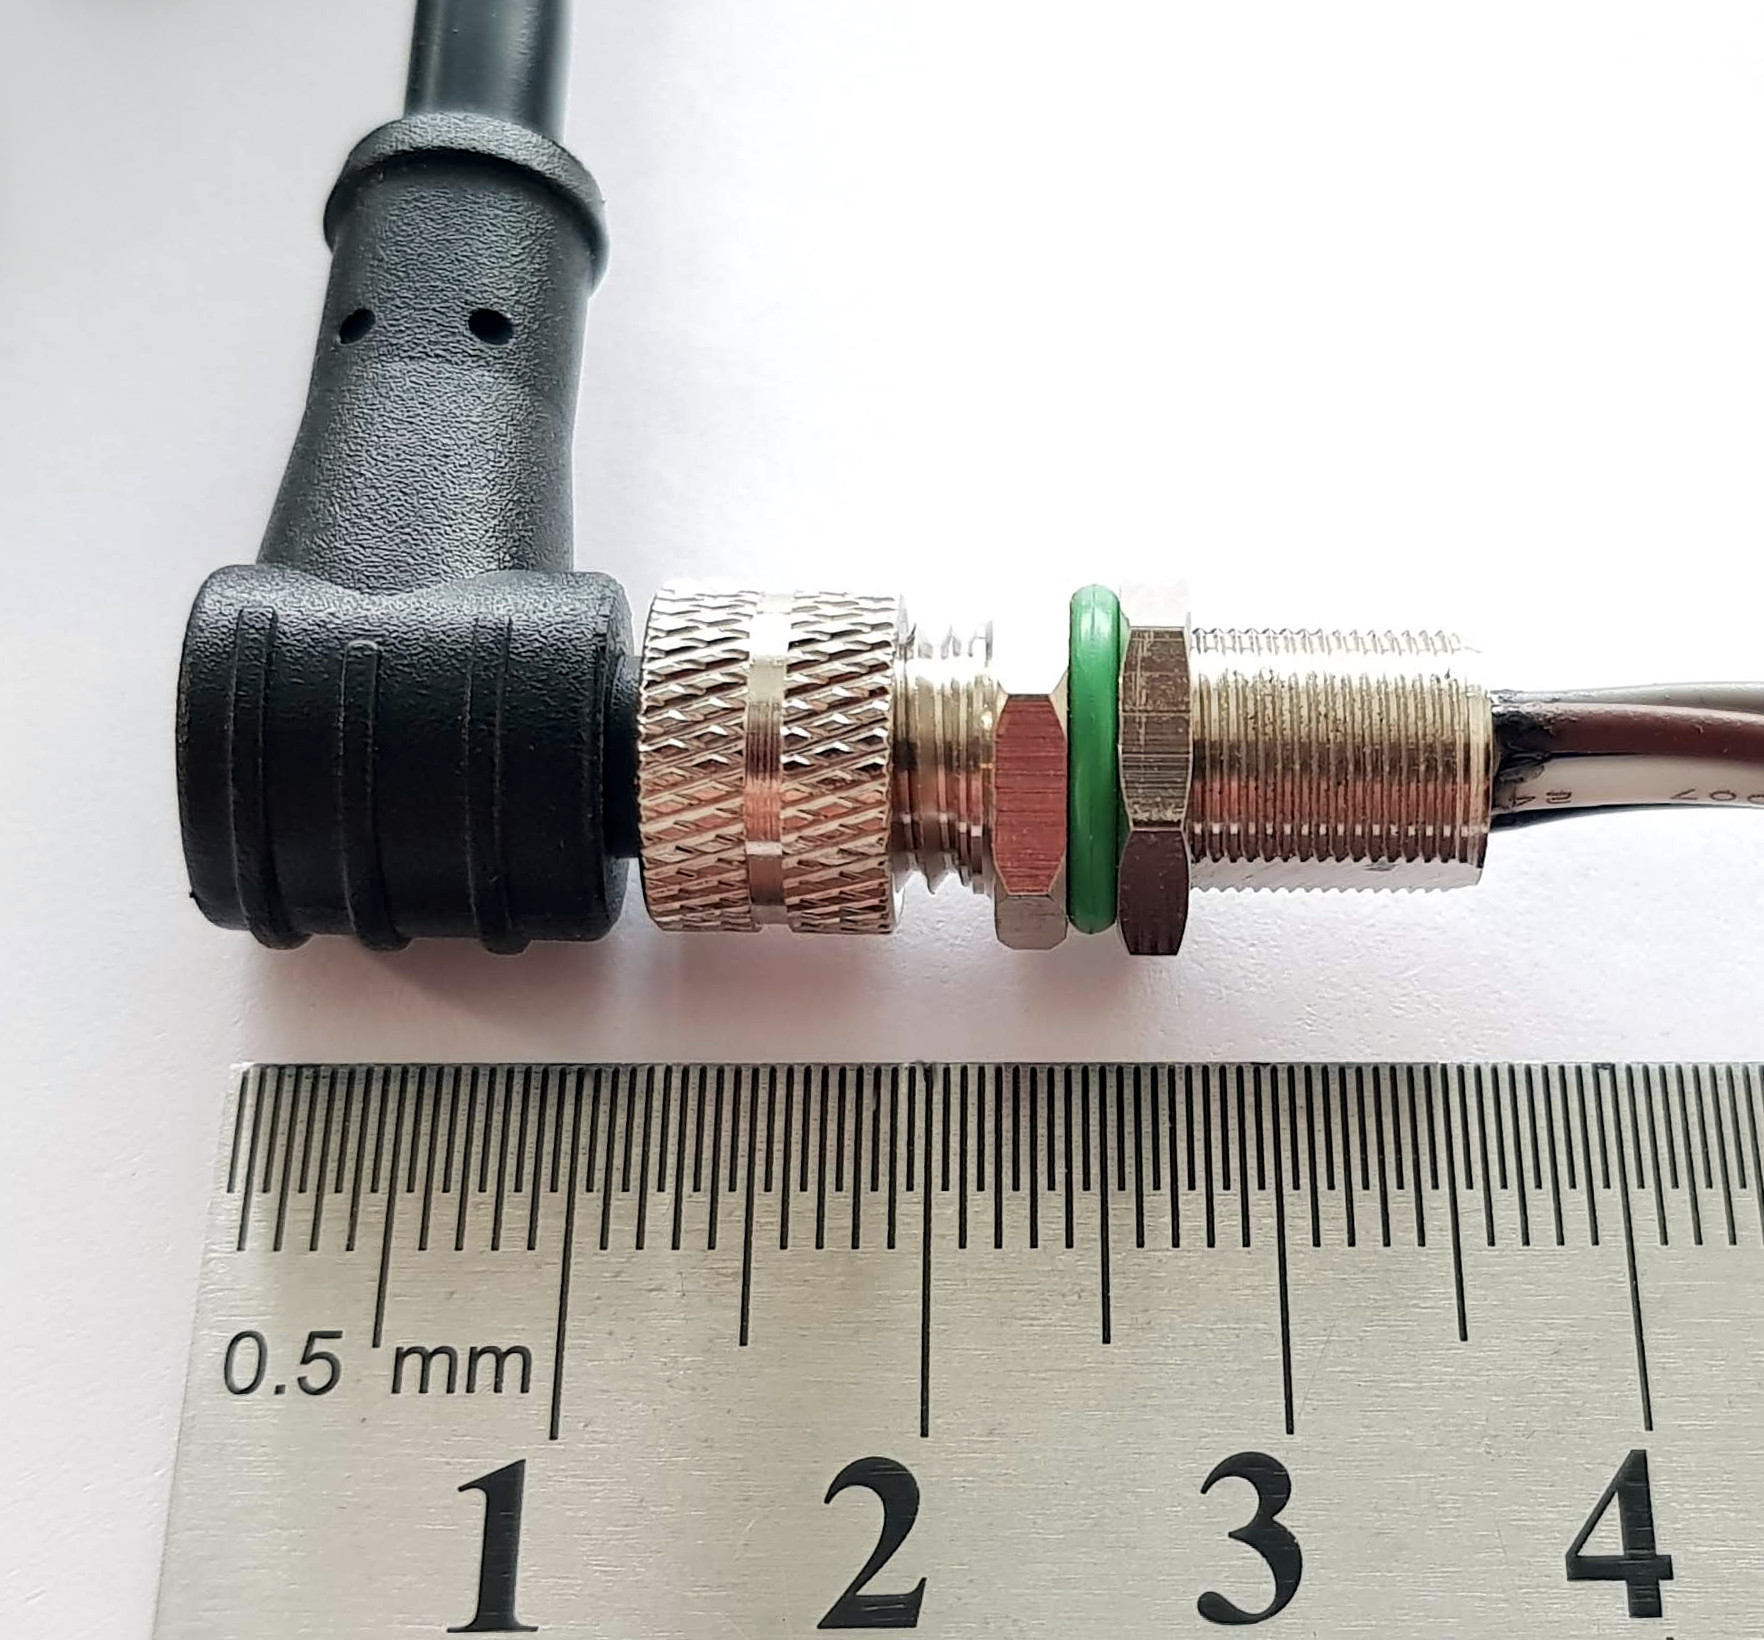
\includegraphics[width=0.35\textwidth]{m8_connector_pair_assembled}\\
    Female socket cable connector, male plug device connector, and the assembled pair.
    \caption{UCANPHY M8 connectors\label{fig:connector_m8}}
\end{figure}

\clearpage  % Enforce \clearpage because the text here is very graphics-heavy and may be hard to read otherwise
\section{UCANPHY Micro}

The UCANPHY Micro connector is intended for weight- and space-sensitive applications.
It is a board-level connector, meaning that it is installed on the PCB rather than on the panel.

The Micro connector is compatible with the Dronecode Autopilot Connector Standard.
This connector type is recommended for small UAV and nanosatellites.
It is also the recommended connector for attaching external panel-mounted connectors
(such as the M8 or D-Sub types) to the PCB inside the enclosure.

{
\NoLeftSkip
\begin{UAVCANCompactTable}{|X X|}
    Advantages & Disadvantages \\
    \begin{itemize}
        \item Extremely compact, low-profile. The PCB footprint is under 9$\times$5 millimeters.
        \item Secure positive lock ensures that the connection will not self-disconnect when exposed to vibrations.
        \item Low cost.
    \end{itemize}
    &
    \begin{itemize}
        \item Board-level connections only. No panel-mounted options available.
        \item No shielding available.
        \item Not suitable for safety-critical hardware.
    \end{itemize}
\end{UAVCANCompactTable}
}

The UCANPHY Micro connector is based on the proprietary \textbf{JST GH 4-circuit} connector type\footnote{%
    The top-entry type is not PCB-footprint-compatible with the side-entry type -- its pin ordering is reversed.
    The wire-side pinout, however, is compatible, so both types can be used interchangeably as long
    as their PCB footprints are correct.
}.

The CAN physical layer standard that can be used with this connector type is ISO 11898-2.

Devices that deliver power to the bus are required to provide 4.9--5.5 V on the bus power line, 5.0 V nominal.
Devices that are powered from the bus should expect 4.0--5.5 V on the bus power line.
The current shall not exceed 1 A per connector.

Table~\ref{table:connector_micro_pinout} documents the pinout specification for the
UCANPHY Micro connector type.
The suitable wire type is \#30 to \#26 AWG, outer insulation diameter 0.8--1.0 mm, multi-strand.
Wires ``CAN high'' and ``CAN low'' shall form a twisted pair.

\begin{UAVCANSimpleTable}{UCANPHY Micro connector pinout}{|l l X|}\label{table:connector_micro_pinout}
    \# & Function           & Note \\
    1  & Bus power supply   & 5 V nominal. See the power supply requirements. \\
    2  & CAN high           & Twisted with ``CAN low'' (pin 3). \\
    3  & CAN low            & Twisted with ``CAN high'' (pin 2). \\
    4  & Ground             & \\
\end{UAVCANSimpleTable}

\begin{figure}[hbt]
    \centering
    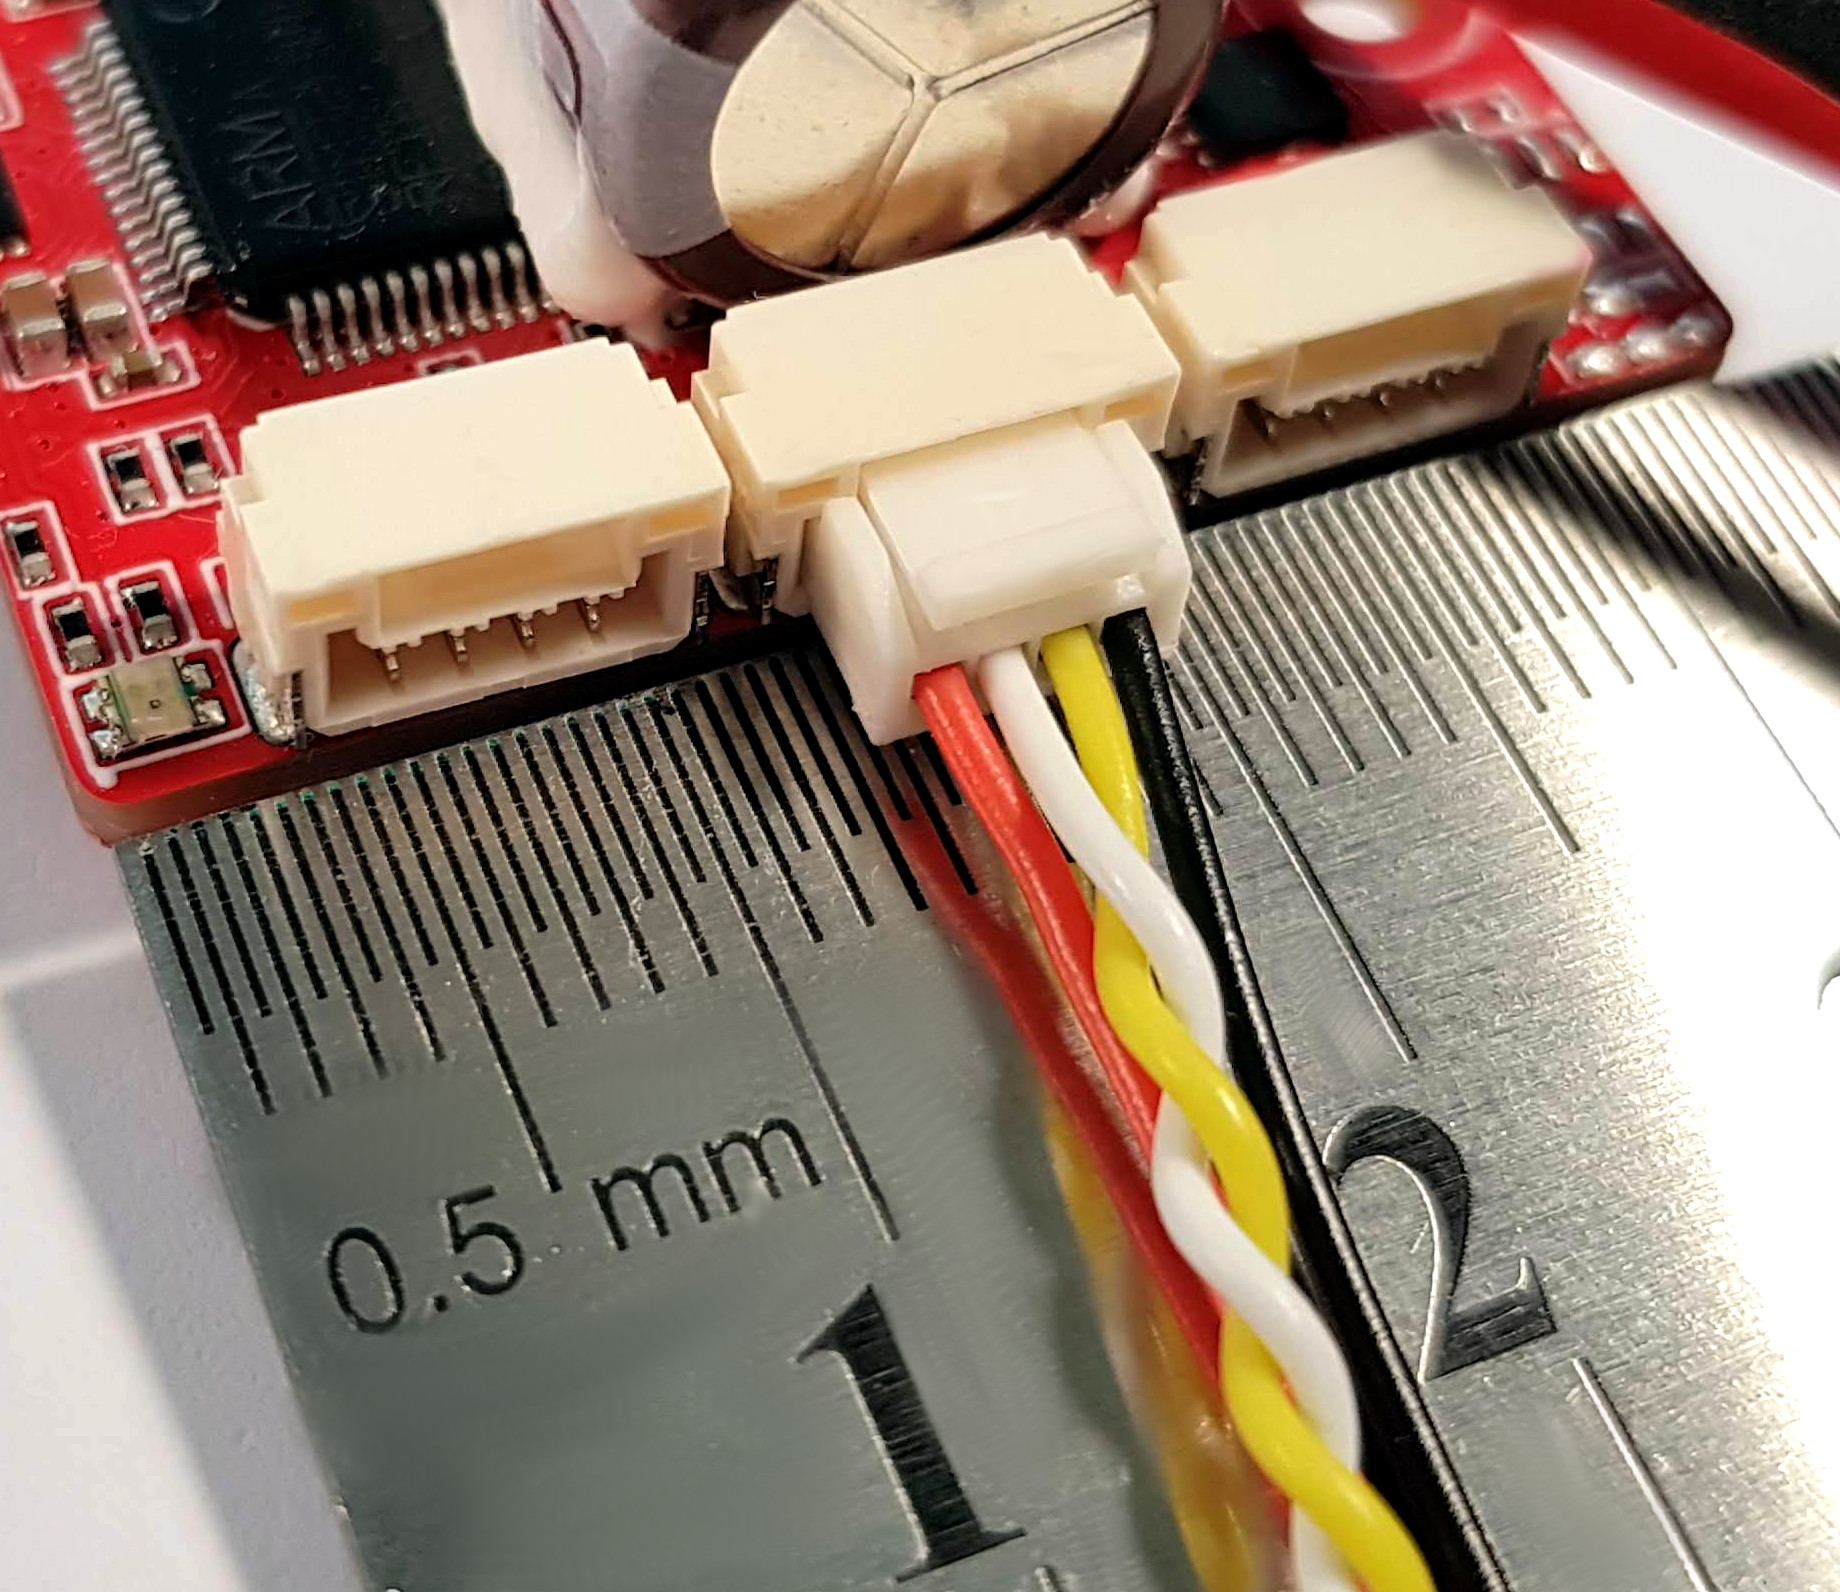
\includegraphics[width=0.35\textwidth]{jst_gh_connectors}
    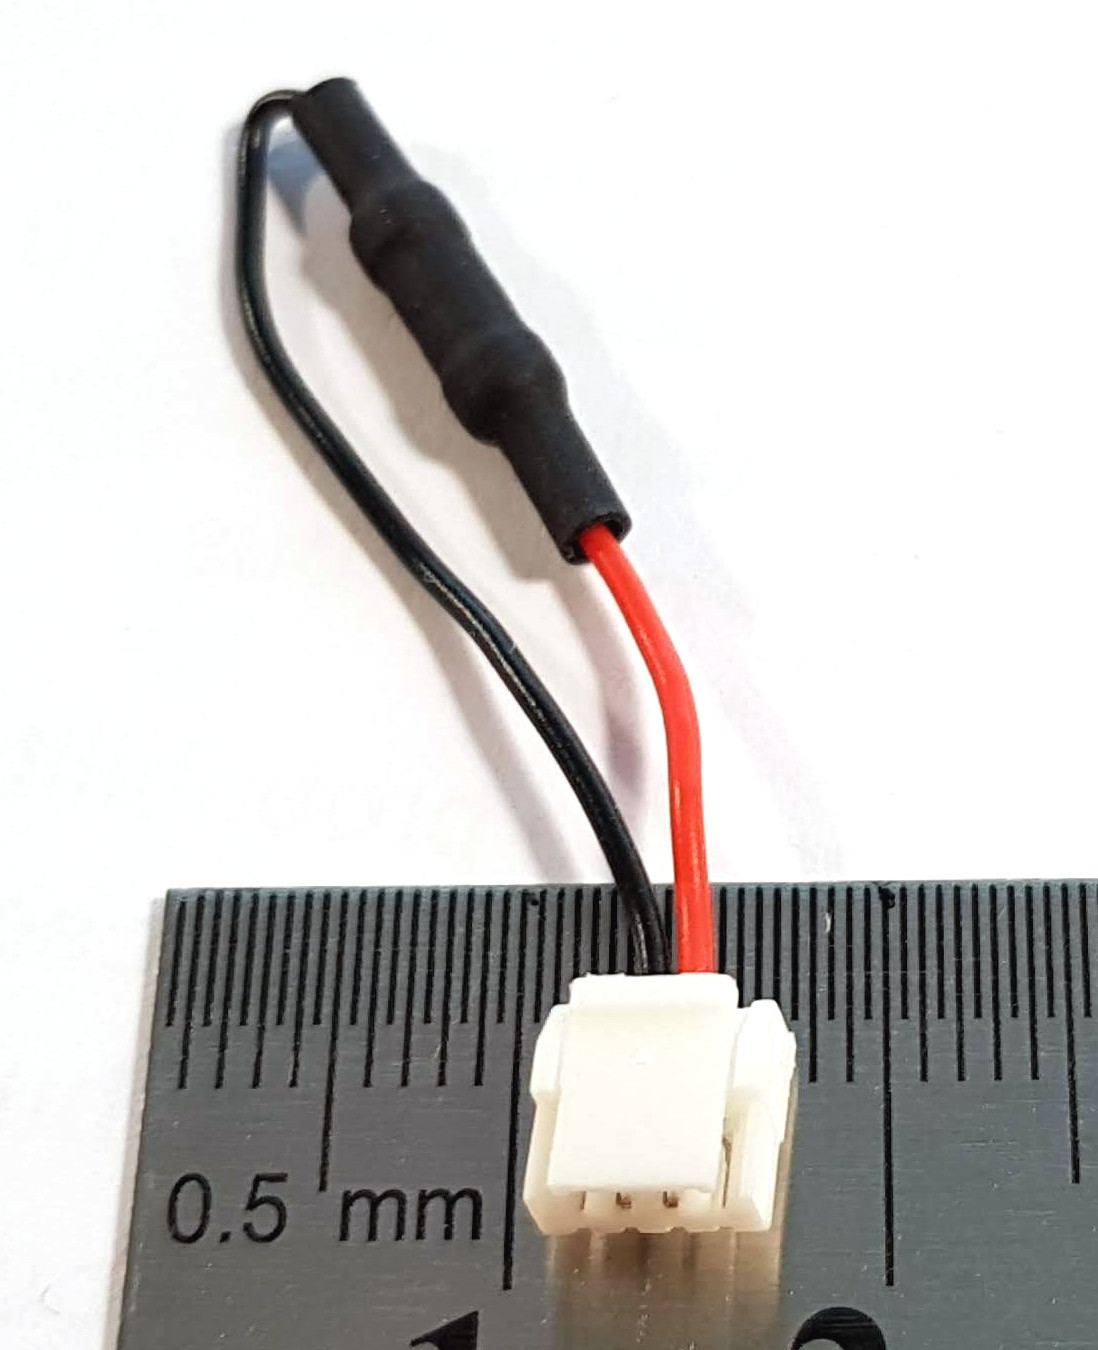
\includegraphics[width=0.30\textwidth]{jst_gh_termination_plug}\\
    Right-angle connector with a twisted pair cable connected; a $120\Omega{}$ termination plug.
    \caption{UCANPHY Micro connectors \label{fig:connector_micro}}
\end{figure}

\chapter{Integrated power supply network}\label{sec:power}

Integration of the power distribution functionality with the communication infrastructure
removes the need for a dedicated power distribution network,
which has the potential to simplify the system design and reduce the complexity and weight of the wiring harnesses.
Redundant power supply topologies can be easily implemented on top of a redundant communication infrastructure.

Designs that integrate power distribution with the communication infrastructure should follow the
conventions set out in this section.

\section{Power input}

A node that draws power from the power supply network should protect its power inputs
with an over-current protection circuitry that is capable of disconnecting the input
if the power consumption of the node exceeds its design limits.
This measure is necessary to prevent a short-circuit or a similar failure of an individual node from affecting
other nodes connected to the same power supply network.

In the case of redundant power supply connections where a node is connected to more than one power supply network
concurrently, each such connection should be equipped with a circuit that prevents reverse current flow
from the node into the power supply network.
This measure is necessary to prevent a short-circuit or a similar failure of an individual power supply network
from affecting other power supply networks in the same redundant group.

\begin{figure}[H]
    \centering
    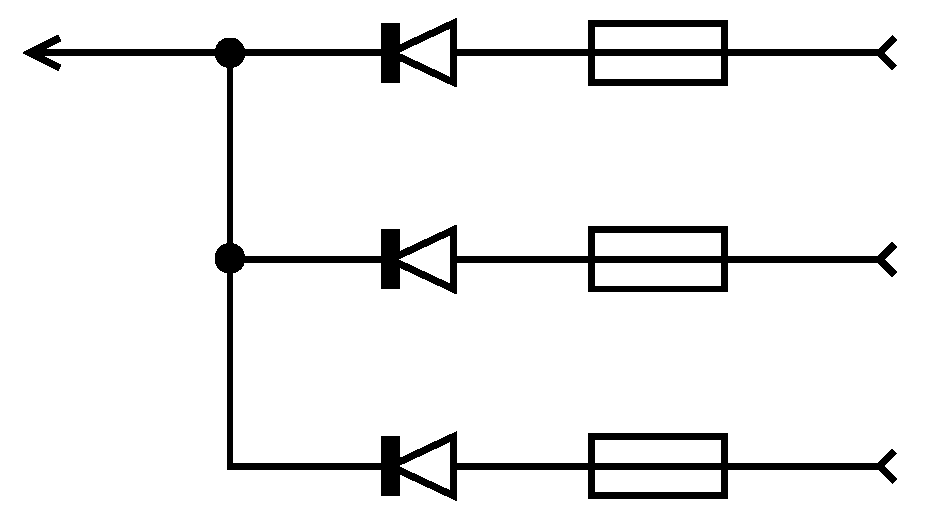
\includegraphics[width=0.3\textwidth]{redundant_power_sink}
    \caption{Redundant power input schematic}
\end{figure}

\section{Power output}

A node that delivers power to the power supply network should equip each of its power outputs
with a circuit that prevents reverse current flow from the power supply network into the node.
This measure is necessary to prevent a short-circuit or a similar failure of the node from affecting
the power supply network.

In the case of redundant power output connections where a node provides power to more than one power supply network
concurrently, each such connection should be equipped with a circuit that is capable of disconnecting the output
if the power consumption per network exceeds the design limits.
This measure is necessary to prevent a short-circuit or a similar failure of an individual power supply network
from affecting other power supply networks in the same redundant group.

\begin{figure}[H]
    \centering
    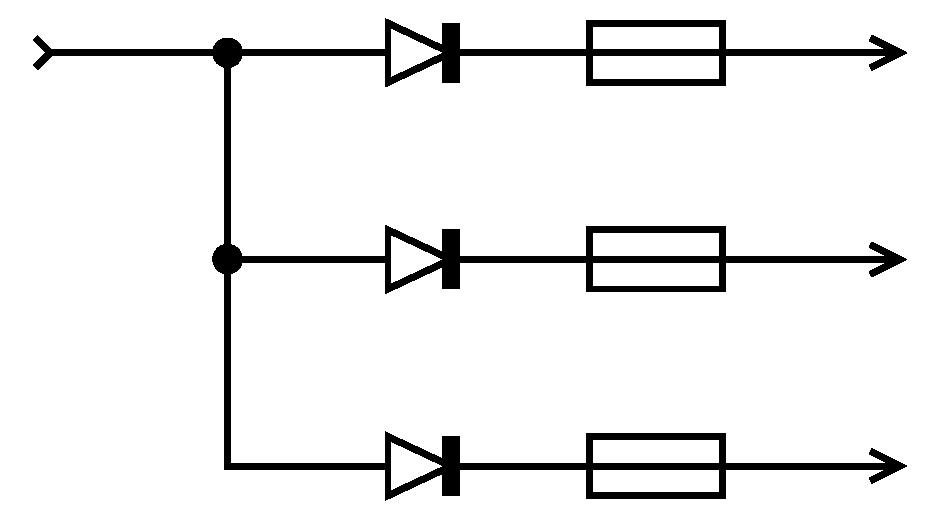
\includegraphics[width=0.3\textwidth]{redundant_power_source}
    \caption{Redundant power output schematic}
\end{figure}


\end{document}
